\documentclass[a4paper,11pt]{article}

%% We can use macros to avoid typing the same thing over and over
\newcommand{\token}[1]{\texttt{<#1>}}
\newcommand{\uC}{{$\mathrm{\mu}$}C }
 \usepackage{tikz}
 \usepackage{tikz-qtree}
 \usepackage{array}
\usepackage{amsmath}
\usepackage{multicol}
\usepackage{listings}
\usepackage{alltt}
\usepackage{hyperref}
\usepackage[lighttt]{lmodern}

%% Simple syntax highlighting for our RTL. Add more keywords here.
\lstset{keywords={Procedure, ADD, SUB, MUL, DIV, LTEQ, LT, EQ, NE, GTEQ, GT,
    Mov, Not, Neg, Jump, Branch, Zero, NonZero, IntConst, GlobalAddress, Store,
    Load, BYTE, INT, Call, ArrayAddress}}

\title{Assignment 4: ICode Generation \\
       Compiler Design Project, 1DL420}
\author{Xiao Yang \and Magnus L{\aa}ng}
\date{\today}
\begin{document}
\maketitle

\section{RTL Design Rationale}
\paragraph{Why flat datatypes?}
Or, in other words, why did we redesign this:

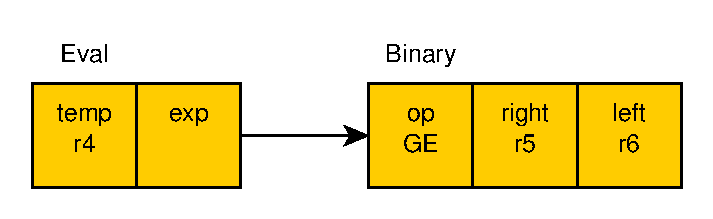
\includegraphics[scale=0.8]{bad}

to this:

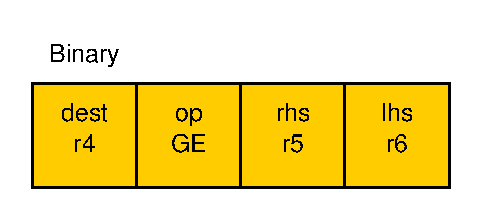
\includegraphics[scale=0.8]{good}

The answer is, we believe the \texttt{RtlExp} pattern facilitates minimal to no
code reuse, and complicates the instruction format, leading to a total of more,
less readable, code.

\paragraph{Why no distinction between locals and temporaries?} Because there is no
reason to. None of the subsequent processing needs to know what is a local and
what is a compiler-introduced temporary, so we cut the information away.

\paragraph{Why having regs $1,\, \dots,\, n$ be the $n$ formals?} Again, this is a
simplication of the format that for example makes it easier to identify what is
a reference to a formal (when required), without losing any expressiveness of
the language.

\paragraph{Why \texttt{\textbf{ArrayAddress}}} instead of \texttt{FP}?] To simplify
adding additional offsets to the array area without generating additional
add-instructions or requiring data-flow optimisations to remove them. None of
the use-cases of FP that we considered is not covered by
\texttt{\textbf{ArrayAddress}}.

Also, unless special cases was added to the code generator, FP would have to be
stored in the stack frame together with all the other locals and temporaries (at
MIPS generation time, that is).

\paragraph{Why did we remove the empty interfaces?} There was no reason to keep
them. Since they were empty, they did not simplify anything, nor did they give
us any type guarantees for what instances might be.

We have no common interface (as in methods) of all our instructions except for
\texttt{toString}, which is provided by \texttt{Object} anyway.

\paragraph{But you could have added an enum of all the instruction types, and added
  a \texttt{getType} method to \texttt{RtlInsn}!} We considered that, but we
would have to combine that with either
\begin{itemize}
\item casts to the subtypes, which we needed anyway.
\item adding methods to \texttt{RtlInsn} that are only supported by a subset of
  instructions, which is terrible because incorrect assumptions about which
  methods are supported won't be caught by the type system.
\end{itemize}

\newpage
\appendix
% Puts the Appendix [letter] in all headings, and not just section headings,
% disabled for now
%% \renewcommand\thesection{Appendix \Alph{section}} %% Add the word ``Appendix'' to the numbering

\section{RTL Documentation}
This documentation is also distributed with the source code, in the
\path{doc/RTL.md} file.

%% Autogenerated from doc/RTL.md with ``kramdown'' tool, do not manually edit.
%% Autogenerated from doc/RTL.md with ``kramdown'' tool, do not manually edit.
\hypertarget{rtl}{}\label{rtl}

RTL operates on a register machine with an infinite amount of
registers. The registers are identified by integer numbers starting
with zero. Register zero is reserved for the return value of the
current procedure. Registers 1 through \emph{n} are the parameters to the
current \emph{n}-ary fuction.

All registers are associated with a type, described by the \emph{RtlType}
enumeration, having one of the following values.

\begin{verbatim}Int, Byte
\end{verbatim}

The size of an {\tt Int} is 4 bytes.

In addition to the registers, each procedure has a certain, specified
per procedure, number of bytes of stack space available for use. The
code aquires the address to this stack space using the {\tt ArrayAddress}
instruction.

\subsection{Instructions}\hypertarget{instructions}{}\label{instructions}

These are the available instructions in the RTL.

\subsubsection{Binary}\hypertarget{binary}{}\label{binary}

\begin{verbatim}Binary(Dest, BinOp, Lhs, Rhs)
\end{verbatim}

Computes a binary instruction that acts on two registers \emph{Lhs} and
\emph{Rhs}, and puts the result in a third register \emph{Dest}.

The \emph{BinOp} enumeration can have the following values.

\begin{verbatim}Add, Sub, Mul, Div, Gt, Lt, GtEq, LtEq, Eq, Ne
\end{verbatim}

The instruction is sometimes pretty-printed as

\begin{verbatim}Dest <- BinOp Lhs, Rhs
\end{verbatim}

\subsubsection{Unary}\hypertarget{unary}{}\label{unary}

Another instruction is {\tt Unary}:

\begin{verbatim}Unary(Dest, UnOp, Arg)
\end{verbatim}

Computes a unary operation that acts on a register \emph{Arg} and puts the
result in a register \emph{Dest}.

The \emph{UnOp} enumeration can have the following values.

\begin{verbatim}Not, Neg, Mov
\end{verbatim}

The instruction is sometimes pretty-printed as

\begin{verbatim}Dest <- UnOp Arg
\end{verbatim}

\subsubsection{Load}\hypertarget{load}{}\label{load}

The {\tt Load} instruction loads a value of type \emph{RtlType} from a memory
address stored in a register \emph{Addr} and writes the loaded value into
register \emph{Dest}.

\begin{verbatim}Load(Dest, RtlType, Addr)
\end{verbatim}

The instruction is sometimes pretty-printed as

\begin{verbatim}Dest <- Load RtlType Addr
\end{verbatim}

\subsubsection{Store}\hypertarget{store}{}\label{store}

The {\tt Store} instruction writes a value of type \emph{RtlType} stored in a
register \emph{Val} to a memory addres stored in register \emph{Addr}.

\begin{verbatim}Store(Addr, RtlType, Val)
\end{verbatim}

The instruction is sometimes pretty-printed as

\begin{verbatim}Addr <- Store RtlType Val
\end{verbatim}

\subsubsection{ArrayAddress}\hypertarget{arrayaddress}{}\label{arrayaddress}

The {\tt ArrayAddress} instruction computes a memory address that is
\emph{Offset} bytes after the memory location in the stack frame where
array locals are stored into a register \emph{Dest}. Note that \emph{Offset} is
an non-negative integer constant.

\begin{verbatim}ArrayAddress(Dest, Offset)
\end{verbatim}

The instruction is sometimes pretty-printed as

\begin{verbatim}Dest <- ArrayAddress Offset
\end{verbatim}

\subsubsection{GlobalAddress}\hypertarget{globaladdress}{}\label{globaladdress}

The {\tt GlobalAddress} instruction loads the memory address of a global
variable or constant with name \emph{Name} into a register \emph{Dest}.

\begin{verbatim}GlobalAddress(Dest, Name)
\end{verbatim}

The instruction is sometimes pretty-printed as

\begin{verbatim}Dest <- GlobalAddress Name
\end{verbatim}

\subsubsection{IntConst}\hypertarget{intconst}{}\label{intconst}

The {\tt IntConst} instruction loads an integer constant \emph{Const} into a
register \emph{Dest}.

\begin{verbatim}IntConst(Dest, Const)
\end{verbatim}

The instruction is sometimes pretty-printed as

\begin{verbatim}Dest <- IntConst Const
\end{verbatim}

\subsubsection{Label}\hypertarget{label}{}\label{label}

The {\tt Label} instruction has no side effects, but defines a location in
the program code that is identified by a string \emph{name}, and may be the
target of control flow instructions. The name must be unique in the
entire program, and may not clash with the names of functions or
global variables.

\begin{verbatim}Label(Name)
\end{verbatim}

The instruction is sometimes pretty-printed as

\begin{verbatim}Name:
\end{verbatim}

\subsubsection{Branch}\hypertarget{branch}{}\label{branch}

The {\tt Branch} instruction diverts control flow to after a {\tt Label}
instruction with name \emph{Name} in the same procedure based on the value
of the register \emph{Cond}.

\begin{verbatim}Branch(Name, Mode, Cond)
\end{verbatim}

The \emph{Mode} enumeration defines what values of the register \emph{Cond} that
causes the control flow to be diverted.

\begin{verbatim}Zero, NonZero
\end{verbatim}

The instruction is sometimes prettyprinted as

\begin{verbatim}Branch Name, Mode, Cond
\end{verbatim}

\subsubsection{Jump}\hypertarget{jump}{}\label{jump}

The {\tt Jump} instruction unconditinally transfers control flow to after a
{\tt Label} instructiom with name \emph{Name} in the same procedure.

\begin{verbatim}Jump(Name)
\end{verbatim}

The instruction is sometimes prettyprinted as

\begin{verbatim}Jump Name
\end{verbatim}

\subsubsection{Call}\hypertarget{call}{}\label{call}

The {\tt Call} instruction calls another procedure with the name \emph{Name},
sending the values of the registers \emph{Args} as arguments, placing the
return value in register \emph{Dest}.

\begin{verbatim}Call(Dest, Name, Args)
\end{verbatim}

The \emph{Dest} parameter may be -1, signifying that the return value (if
any) should be discarded. In this form, the instruction may be
constructed as

\begin{verbatim}Call(Name, Args)
\end{verbatim}

The instruction is sometimes prettyprinted as

\begin{verbatim}Dest <- Call Name [Arg [, Arg...]]

Call Name [Arg [, Arg...]]
\end{verbatim}


\section{Sample RTL for Test Files}
\subsection{\texttt{quiet/lexer/l05.c}}
\begin{lstlisting}
Procedure main
  Argument count: 0
  Stack frame size: 0
  Register types:
    RV: INT
    r1: INT
    r2: INT
    r3: INT
    r4: INT
    r5: INT
    r6: INT
    r7: INT
    r8: INT
    r9: INT
    r10: INT
    r11: INT
    r12: INT
    r13: INT
    r14: INT
    r15: INT
    r16: INT
    r17: INT
    r18: INT
    r19: INT
    r20: INT
    r21: INT
    r22: INT
    r23: INT
    r24: INT
    r25: INT
    r26: INT
    r27: INT
    r28: INT
    r29: INT
    r30: INT
    r31: INT
    r32: INT
  Instructions:
      r3 <- IntConst 1
      r4 <- IntConst 3
      r4 <- Not r4
      r2 <- NE r3, r4
      r6 <- IntConst 4
      r5 <- Mov r6
      Branch main.andshortcircut, NonZero, r5
      r7 <- IntConst 6
      r5 <- Mov r7
    main.andshortcircut:
      r10 <- IntConst 7
      r11 <- IntConst 8
      r9 <- MUL r10, r11
      r12 <- IntConst 10
      r8 <- ADD r9, r12
      r15 <- IntConst 11
      r16 <- IntConst 12
      r14 <- SUB r15, r16
      r18 <- IntConst 12
      r19 <- IntConst 16
      r17 <- DIV r18, r19
      r13 <- ADD r14, r17
      r22 <- IntConst 17
      r23 <- IntConst 18
      r21 <- LTEQ r22, r23
      r24 <- IntConst 20
      r24 <- Neg r24
      r20 <- LT r21, r24
      r26 <- IntConst 21
      r27 <- IntConst 22
      r25 <- EQ r26, r27
      r1 <- Mov r25
      r30 <- IntConst 25
      r31 <- IntConst 27
      r29 <- GTEQ r30, r31
      r32 <- IntConst 28
      r28 <- GT r29, r32
    main.exit:
\end{lstlisting}

\subsection{\texttt{quiet/rtl/r01.c}}
\begin{lstlisting}
y: 1
x: 4
Procedure main
  Argument count: 0
  Stack frame size: 0
  Register types:
    RV: INT
    r1: INT
    r2: BYTE
    r3: INT
    r4: INT
    r5: INT
    r6: INT
    r7: INT
    r8: INT
  Instructions:
      r3 <- IntConst 42
      r4 <- GlobalAddress x
      r4 <- Store INT r3
      r5 <- IntConst 43
      r6 <- GlobalAddress y
      r6 <- Store BYTE r5
      r7 <- IntConst 65
      r1 <- Mov r7
      r8 <- IntConst 10
      r2 <- Mov r8
    main.exit:
\end{lstlisting}

\subsection{\texttt{quiet/rtl/r02.c}}
\begin{lstlisting}
Procedure f
  Argument count: 2
  Stack frame size: 0
  Register types:
    RV: INT
    r1: INT
    r2: INT
    r3: INT
  Instructions:
      r3 <- ADD r1, r2
      RV <- Mov r3
      Jump f.exit
    f.exit:
Procedure main
  Argument count: 0
  Stack frame size: 0
  Register types:
    RV: INT
    r1: INT
    r2: INT
    r3: INT
  Instructions:
      r1 <- IntConst 2
      r2 <- IntConst 3
      r3 <- Call f r1, r2
    main.exit:
\end{lstlisting}

\subsection{\texttt{quiet/rtl/r03.c}}
\begin{lstlisting}
a: 40
Procedure main
  Argument count: 0
  Stack frame size: 12
  Register types:
    RV: INT
    r1: INT
    r2: INT
    r3: INT
    r4: INT
    r5: INT
    r6: INT
    r7: INT
    r8: INT
    r9: INT
    r10: INT
    r11: INT
    r12: INT
    r13: INT
    r14: INT
    r15: INT
    r16: INT
  Instructions:
      r2 <- GlobalAddress a
      r3 <- IntConst 5
      r4 <- IntConst 4
      r4 <- MUL r4, r3
      r4 <- ADD r4, r2
      r4 <- Load INT r4
      r5 <- IntConst 7
      r1 <- ADD r4, r5
      r6 <- GlobalAddress a
      r7 <- IntConst 3
      r8 <- IntConst 4
      r8 <- MUL r8, r7
      r8 <- ADD r8, r6
      r8 <- Store INT r1
      r10 <- ArrayAddress 0
      r11 <- IntConst 5
      r12 <- IntConst 1
      r12 <- MUL r12, r11
      r12 <- ADD r12, r10
      r12 <- Load BYTE r12
      r13 <- IntConst 7
      r9 <- ADD r12, r13
      r14 <- ArrayAddress 0
      r15 <- IntConst 3
      r16 <- IntConst 1
      r16 <- MUL r16, r15
      r16 <- ADD r16, r14
      r16 <- Store BYTE r9
    main.exit:
\end{lstlisting}

\subsection{\texttt{quiet/rtl/r04.c}}
\begin{lstlisting}
Procedure f
  Argument count: 1
  Stack frame size: 0
  Register types:
    RV: INT
    r1: INT
  Instructions:
    f.exit:
Procedure main
  Argument count: 0
  Stack frame size: 8
  Register types:
    RV: INT
    r1: INT
  Instructions:
      r1 <- ArrayAddress 0
      Call f r1
    main.exit:
\end{lstlisting}

\subsection{\texttt{quiet/rtl/r05.c}}
\begin{lstlisting}
a: 40
Procedure f
  Argument count: 1
  Stack frame size: 0
  Register types:
    RV: INT
    r1: INT
    r2: INT
    r3: INT
    r4: INT
    r5: INT
    r6: INT
    r7: INT
  Instructions:
      r3 <- IntConst 5
      r4 <- IntConst 4
      r4 <- MUL r4, r3
      r4 <- ADD r4, r1
      r4 <- Load INT r4
      r5 <- IntConst 7
      r2 <- ADD r4, r5
      r6 <- IntConst 3
      r7 <- IntConst 4
      r7 <- MUL r7, r6
      r7 <- ADD r7, r1
      r7 <- Store INT r2
    f.exit:
Procedure main
  Argument count: 0
  Stack frame size: 0
  Register types:
    RV: INT
    r1: INT
  Instructions:
      r1 <- GlobalAddress a
      Call f r1
    main.exit:
\end{lstlisting}

\end{document}
